\chapter{Utilizas magnitudes y números reales}

\section{Números reales}

\subsection*{Resumen}

Los números reales (designados por $\mathbb R$) pueden ser representatos como
puntos sobre una recta.

\begin{center}
\begin{tikzpicture}
  \draw (-3,0) --(3,0);
  \path (-4,0) node (minf) {$\ldots$};
  \path (4,0) node (inf) {$\ldots$};
  \draw (-1,-.1) --(-1,.1);
  \draw (-2,-.1) --(-2,.1);
  \draw (0,-.1) --(0,.1);
  \draw (1,-.1) --(1,.1);
  \draw (2,-.1) --(2,.1);
  \path (0,.5) node (n0) {$0$};
  \path (1,.5) node (n1) {$1$};
  \path (2,.5) node (n2) {$2$};
  \path (-1,.5) node (nm1) {$-1$};
  \path (-2,.5) node (nm2) {$-2$};
\end{tikzpicture}
\end{center}

Los números naturales (designados por $\mathbb N$) son $0, 1, 2, 3, \ldots$. Si
además incluyemos los números negativos, obtenemos los números enteros
(designados por $\mathbb Z$: $\ldots -3, -2, -1, 0, 1, 2, 3, \ldots$).
Los números de la forma
$\frac{p}{q}$ donde $p \in \mathbb Z$ y $q \in \mathbb N \setminus \{0\}$ se
llaman los racionales (designados por $\mathbb Q$). En particular si considemos
los racionales donde $q=10^n$ para algun $n \in \mathbb N$, obtenemos los
número decimales como $-494.1627$.
Los reales que no son racionales se llaman números irracionales.

\begin{center}
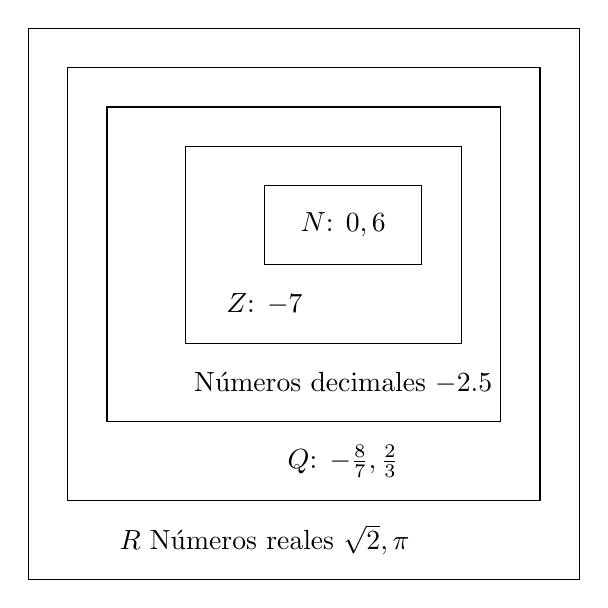
\begin{tikzpicture}
  \draw (0,0) rectangle(7,7);
  \path (3,0.5) node (R) {$\mathbb R$ Números reales $\sqrt{2}, \pi$};
  \draw (.5,1) rectangle(6.5,6.5);
  \path (4,1.5) node (Q) {$\mathbb Q$: $-\frac{8}{7}, \frac{2}{3}$};
  \draw (1,2) rectangle(6,6);
  \path (4,2.5) node (D) {Números decimales $-2.5$};
  \draw (2,3) rectangle(5.5,5.5);
  \path (3,3.5) node (Z) {$\mathbb Z$: $-7$};
  \draw (3,4) rectangle(5,5);
  \path (4,4.5) node (N) {$\mathbb N$: $0, 6$};
\end{tikzpicture}
\end{center}

\subsection*{Ejemplos}

\begin{enumerate}
\item $364$ es un número natural.
\item $-36$ es un número entero (negativo) pero no es un número natural.
\item $0.8$ es un número decimal pero no es entero.
\item $\frac{1}{3}$ es un numero racional pero no es un número decimal.
\item $\sqrt{2}$ es un numero real pero no es un número racional (ejercicio 2).
\end{enumerate}

\subsection*{Ejercicio 1}

Calcular $3n$ y $3{(n+1)}$ para $n = 3, 33, 333, 3333, \ldots$ etc y $10^m$ para
$m = 0, 1, 2, 3, \ldots$.

Suponemos que $\frac{1}{3}$ se puede escribir como un decimal
$\frac{n}{10^m}$ donde $n \in \mathbb N$ y $m \in \mathbb N$. ¿Es eso posible?

\subsection*{Ejercicio 2}

Clasifiar los ńumeros reales siguientes (enteros, racionales...)

\begin{enumerate}
\item $6$
\item $-2$
\item $2.5$
\item $-7.0$
\item $\frac{3}{2}$
\item $-\frac{1}{3}$
\item $\frac{16}{8}$
\item $\sqrt{2}$
\item $\sqrt{49}$
\item $\sqrt{\frac{16}{25}}$
\item $\sqrt[3]{0.125}$
\end{enumerate}

\subsection*{Ejercicio 3 (difícil antes del capítulo IV)}

Si $n$ es un entero, verifia que ${(2n+1)}^2 = 2{(2n^2+2n)} + 1$ y que
${2n}^2 = 2{(2n)}$. Cuál es la relación entre la paridad de un entero y
de su cuadrado?

Consideramos $p \in \mathbb Z$ y $q \in {\mathbb N} \setminus \{0\}$
tal que $\sqrt{2} = \frac{p}{q}$ y $q$ el más pequeño posible.
Muestrar que $p^2$ es un número par y entonces $p$ también.

Si escribimos $p = 2n$, muestrar que $q^2 = 2n^2$ y entonces $q$ es par.
Encuentra $p'$ y $q'$ tal que $q' < q$ y $\sqrt{2} = \frac{p'}{q'}$,
contradiciendo la hipótesis original.

\subsection*{Ejercicio 4}

Ubica en la recta numérica de números reales los números siguientes: $0, 1, 8,
0.25, -4, \frac{9}{4}, \frac{10}{3}, -\sqrt{2}$.

\subsection*{Ejercicio 5 (introducción informal a los números complejos)}

Suponemos que existe un número $i$ tal que $i^2 = -1$ y consideramos el
conjunto de los complejos
$\mathbb{C} = \left\{ a + ib, a \in \mathbb{R}, b \in \mathbb{R} \right\}$.
Si $z = a + ib$, $a$ es parte real y $b$ la parte imaginaria. Si $a = 0$,
$z$ es dicho número imaginario puro.
El conjugado de $z$ es $\bar{z} = a - i b$ y el módulo de $z$ es
${|z|} = \sqrt{a^2 + b^2}$. El complejo $z \neq 0$
puede ser representado en un plano de la manera siguiente:

\begin{center}
\begin{tikzpicture}
  \draw (0,0) node[left] {$0$} circle (2);
  \draw[style=dashed,color=gray] (0,0) circle (3);
  \draw[color=red] (0,0) -- (0.75,1.299038105676657) node[left] {$\rho$} --(1.5,2.598076211353315) node[right] {$z=a+ib$};
  \draw[->] (0,0) -- (4,0);
  \draw[->] (0,0) -- (0,4);
  \path (2,0) node[right] {$1$};
  \path (0,2) node[above] {$i$};
  \draw[style=dashed,color=blue] (1.5,2.598076211353315) -- (1.5,0) node[right] {$a$};
  \draw[style=dashed,color=blue] (1.5,2.598076211353315) -- (0,2.598076211353315) node[above] {$b$};
  \draw[color=green] (.5,0) arc (0:60:.5) node[right] {$\varphi$};
\end{tikzpicture}
\end{center}

\begin{enumerate}
\item ¿Cómo definir la suma, resta, producto de números complejos?
\item  $z \bar{z}$ y deducir un número $z'$ tal que $z z' = 1$. ¿Como definir
  el inverso de un número complejo y la división de dos complejos?
\item Muestrar que para cada número real $r \neq 0$, hay dos complejos
  $z_1 \neq z_2$ tal que $z_1^2 = z_2^2 = r$. ¿Que decir de esos números segun
  el signo de $r$?
\item En la representación gráfica, $\rho$ es el módulo de $z$ y el angulo
  $\varphi$ es llamado el argumento. Expresar $a, b$
  en función de $\rho$ y $\varphi$.
\item Cómo interpretar gráficamente la suma, resta y conjugación de complejos?
\item Recordar las formulas para el coseno y seno de la suma de dos ángulos.
  Si $z_1, z_2$ tienen módulos y argumentos $\rho_1, \varphi_1$ y
  $\rho_2, \varphi_2$, ¿Cómo se expresa el producto $z_1 \times z_2$ en función
  de esos parametros? ¿Cómo interpretar gráficamente el producto de dos
  complejos?
\item Deducir que para cada número real $r \neq 0$ sólo hay dos $z$ tal
  que $z^2 = r$ . ¿Que decir de $r=0$?
\end{enumerate}

\section{Operaciones}

\subsection*{Resumen}

Las operaciones vistas para los números positivos existen también para
los reales:

\begin{enumerate}
\item Suma: si $p, q$ son números positivos, tenemos
  $p + -q = p - q$, $-p + q = q - p$ y $-p + -q = -{(p+q)}$.
\item Resta: si $p, q$ son números positivos, tenemos
  $p - -q = p + q$, $-p - q = -{(p + q)}$ y $-p - -q = q - p = -{(p - q)}$.
\item Multiplicación: si $p, q$ son números positivos, tenemos
  $p \times -q = -p \times q = -{(p \times q)}$ y
  $-p \times -q = p \times q$
\item División: $p, q$ son números positivos y $q \neq 0$, tenemos
  $p / -q = -p / q = -{(p / q)}$ y
  $-p / -q = p / q$
\item $p^{-n} = \frac{1}{p^n}$ para $p$ real y $n$ entero.
\item Si $p$ es un número positivo y $n$ es entero,
  ${-p}^{n} = p^n$ si $n$ es par y ${-p}^{n} = -p^n$ si $n$ es impar.
\item $\sqrt[n]{-p} = -\sqrt[n]{p}$ si $n$ es impar y $p$ positivo. No podemos
  definir un tal número real si $n$ es par y $p > 0$.
\end{enumerate}

\subsection*{Ejemplos}

\begin{enumerate}
\item $-1 + -5 = -6$, $5 - 7 = -2$
\item $5 - -6 = 11$, $-7 - 8 = -15$
\item $-2 \times 3 = -6$, $-2 \times -3 = 6$
\item $-8 / 4 = -2$, $-10 / -5 = 2$
\item $2^-3 = \frac{1}{2^3} = \frac{1}{8} = 0.125$, ${(-2)}^{3} = -8$
\item $\sqrt[3]{-27} = -3$
\end{enumerate}

\subsection*{Ejercicio 6}

Calcular:

\begin{enumerate}
\item ${(-1 + 6)} \times {(-2)}^3$
\item $\frac{-5 + -2}{7} + 2$
\item $2 \sqrt[3]{(10 - 11 \times 4 + 14 / 2)}$
\item $8 - \left(\frac{2}{-3}\right)^{-2} + 1$
\end{enumerate}

\subsection*{Ejercicio 7}

El kelvin es la unidad de temperatura del Sistema Internacional de Unidades.

Otras unidades usadas par medir la temperatura son los grados Fahrenheit y
Celcius. Para convertir una tempentura $T$ en kelvin a una tempentura en grado
Fahrenheit, hay que multiplicar $T$ por $\frac{9}{5}$ y restar $459.67$.
Para convertir una tempentura $T$ en grado Celcius a una tempentura $T$ en
kelvin, hay que añadir $273.15$.

Si la temperatura era $59°F$ por la mañana y ha crecido de $5\%$. ¿Cuál es ahora
la temperatura en grado Celcius?

\section{Razones, tasas, proporciones y variaciónes}

\subsection*{Resumen}

Una razón es fracción que compara dos cantidades. Por ejemplo,
tres de cada diez mujeres:
$\frac{3}{10}$, $3:10$, $3$ de $10$. Una tasa es una razón de dos cantidades
diferentes. $100$ kilometros por $2$ horas: $\frac{100}{2}$, $100 : 2$,
$100$ de $2$.

Una proporción es dos razones o fracciones iguales $\frac{a}{b} = \frac{c}{d}$.
$a$ es a $c$ como $b$ es a $d$. Los extremos de la proporción son $a$ y $d$,
mientras $b$ y $c$ son llamados los medios. El producto de los medios es igual
al producto de los extremos: $a d = c b$.

Una variación es la evolución de una variable ```a'' con respecto a otra
``b'', por una razón ``k''. Una variacíon es directa si la primera variable
aumenta cuando la otra aumenta ($a = k \times b$) y inversa si la
primera variable disminuye cuando la otra aumenta ($a = k / b$).

\subsection*{Ejercicio 8}

\begin{enumerate}
\item En una tienda, 1.5kg de tomate cuesta 24MXN. En otra tienda, 300g de
  tomate cuesta 5MXN. ¿Cuál es la mejor compra?
\item Dos botellas de agua cuestan 16.72MXN. ¿Cuantos botellas podemos comprar
  con 50.16MXN?
\item En electricidad, la ley de Ohm relaciona el voltaje $V$, con la carga
  $R$, y la corriente $I$ con la relación $V=RI$. Indicata el tipo de
  variación de $R$ con respecto a $I$.
\end{enumerate}

\section{Soluciones de los ejercicios}

\subsection*{Ejercicio 1}

Obtenemos $9, 99, 9999, 99999$, $12, 102, 1002, 10002$ y
$1, 10, 100, 1000, 10000, \ldots$. Nos damos cuenta de que $10^m$ nunca es divisible
por $3$. Entonces $\frac{1}{3} = \frac{n}{10^m}$ no es posible o tendríamos
$10^m = 3n$.

\subsection*{Ejercicio 2}

\begin{enumerate}
\item $6$ es un número natural.
\item $-2$ es un número entero pero no es natural.
\item $2.5 = \frac{25}{10^1}$ es un número decimal pero no es entero.
\item $-7.0 = -7$ es un número entero pero no es natural.
\item $\frac{3}{2} = 1.5$ es un número decimal pero no es entero.
\item $-\frac{1}{3}$ es un numero racional pero no es decimal por ejercicio 1.
\item $\frac{16}{8} = 2$ es un número natural.
\item $\sqrt{2}$ es un numero real pero no es racional por ejercicio 3.
\item $\sqrt{49} = 7$ es un número natural.
\item $\sqrt{\frac{16}{25}} = \frac{4}{5} = \frac{8}{10^1} = 0.8$ es un número
decimal pero no es entero.
\item $\sqrt[3]{0.125} = 0.5$ es un número decimal pero no es entero.
\end{enumerate}

\subsection*{Ejercicio 3}

${(2n+1)}^2 = {(2n+1)}{(2n+1)} = 4n^2 + 2n + 2n + 1 = 4n^2 + 4n + 1 =
2{(2n^2+2n)} + 1$ y ${2n}^2 = 4n^2 = 2{(2n)}$. Entonces
un entero $N$ es par si y solo si $N^2$ es par.

Si $\sqrt{2} = \frac{p}{q}$, $2 = \frac{p^2}{q^2}$ y entonces
$p^2 = 2q^2$ es par. Por el primer párafo, $p$ es par y se puede escribir
$p = 2n$ para alguno entero $n$.

Ahora, tenemos $2q^2 = {(2n)}^2 = 4n^2$ y entonces $q^2 = 2n^2$ es par.
Aún podemos escribir $q = 2m$ para alguno entero $n$ y finalmente
$\sqrt{2} = \frac{2n}{2m} = \frac{n}{m}$. Si ponemos $p' = n$ y $q' = m$
encontramos una contradición.

\subsection*{Ejercicio 4}

$0.25 = \frac{1}{4}$, $\frac{9}{4} = 2 + \frac{1}{4}$,
$\frac{10}{3} = 3 + \frac{1}{3}$, $-\sqrt{2} \approx -1.414213562373095$

\begin{center}
\begin{tikzpicture}
  \draw (-9,0) --(9,0);
  \draw (1,-.2) --(1,.2);
  \draw (2,-.1) --(2,.1);
  \draw (3,-.1) --(3,.1);
  \draw (4,-.1) --(4,.1);
  \draw (5,-.1) --(5,.1);
  \draw (6,-.1) --(6,.1);
  \draw (7,-.1) --(7,.1);
  \draw (8,-.1) --(8,.1);
  \draw (0,-.2) --(0,.2);
  \draw (-1,-.1) --(-1,.1);
  \draw (-2,-.1) --(-2,.1);
  \draw (-3,-.1) --(-3,.1);
  \draw (-4,-.1) --(-4,.1);
  \draw (-5,-.1) --(-5,.1);
  \draw (-6,-.1) --(-6,.1);
  \draw (-7,-.1) --(-7,.1);
  \draw (-8,-.1) --(-8,.1);
  \path (0,.5) node (n0) {$0$};
  \path (1,.5) node (n1) {$1$};
  \path (2,.5) node (n2) {$2$};
  \path (3,.5) node (n3) {$3$};
  \path (4,.5) node (n4) {$4$};
  \path (-4,.5) node (nm4) {$-4$};

  \draw (0.25,-.1) --(0.25,2);
  \draw (0.5,-.1) --(0.5,.1);
  \draw (0.75,-.1) --(0.75,.1);
  \path (0.25,2.2) node (n025) {$0.25$};

  \draw (2.25,-.1) --(2.25,2);
  \path (2.25,2.2) node (n94) {$\frac{9}{4}$};

  \draw (3.333333333333,-.1) --(3.333333333333,2);
  \draw (3.666666666666,-.1) --(3.666666666666,.1);
  \path (3.333333333333,2.2) node (n103) {$\frac{10}{3}$};

  \draw (-1.414213562373095,-.1) --(-1.414213562373095,2);
  \path (-1.414213562373095,2.2) node (nmsqrt2) {$-\sqrt{2}$};


\end{tikzpicture}
\end{center}

\subsection*{Ejercicio 5 (introducción informal a los números complejos)}

\begin{enumerate}
\item Sean $z = a+ib$ y $z' = a'+ib'$.
  $z + z' = {(a+a')} + i (b+b')$, $z - z' = {(a-a')} + i {(b-b')}$.
  $z \times z' = {a a'} + {i ab'} + {i a'b} + {(ib)(ib')} =
  {(aa' - bb')} + i {(ab' + a'b)}$
\item $z \bar{z} = a^2 + b^2 + i {(ab - ab)} = {|z|}^2$
  Entonces si $z' = \frac{\bar{z}}{{|z|}^2}$, $z z' = 1$. Definimos el inverso
  de $z$ por $z^{-1} = \frac{\bar{z}}{{|z|}^2}$ y
  $\frac{z_1}{z_2} = z_1 z_2^{-1}$.
\item Si $r > 0$ ya sabemos que $z_1 = -\sqrt{r}$ y $z_2 = \sqrt{r}$ convienen.
  Si $r < 0$, notamos que $z_1 = -i\sqrt{r}$ y $z_2 = i\sqrt{r}$ convienen
  tambíen porque $i^2 = -1$. Si $r > 0$ $z_1,z_2$ son reales y si $r < 0$,
  esos son imaginario puro.
\item $a = \rho {\cos(\varphi)}$, $b = \rho {\sin(\varphi)}$
\item La suma y resta se intepretan como suma y resta de vectores. La conjucación como la simetria en el eje $X$.
\item $z_1 z_2 = {\rho_1 \rho_2} \left({\cos(\varphi_1 + \varphi_2)} + i
  {\sin(\varphi_1 + \varphi_2)} \right)$. Entonces el módulo del producto es el
  producto de los modulos y el argumento del producto es la suma de los argumentos.
\item Si $z^2 = r$ y tenemos ${|z|}^2 = {|r|}$ y $2 \varphi \equiv 0 \mod 360°$ ($r > 0$) o $2 \varphi \equiv 180 \mod 360°$ ($r < 0$).
  Entonces $|z| = \sqrt{|r|}$ y $\varphi \equiv 0, 180 \mod 360°$ ($r > 0$)
  o $\varphi \equiv 90, 270 \mod 360°$ ($r < 0$), y esos son los soluciones
  encontradas arriba. Si $z \neq 0$, ${|z|} \neq 0$ y ${|z^2|} =
  {|z|}^2 \neq 0$. Entonces el único complejo tal que $z^2 = 0$ es $z = 0$.
\end{enumerate}

\subsection*{Ejercicio 6}

\begin{enumerate}
\item $-40$
\item $1$
\item $-6$
\item $\frac{27}{4}$
\end{enumerate}

\subsection*{Ejercicio 7}

Hay que trabajar con la temperatura absoluta (en kelvin)!

$59°F$ corresponde a ${(59+459.67)} \times \frac{5}{9} = 288.15$ kelvin.
Si ha crecido de $5\%$, ahora la temperatura es
$288.15 \times \left(1+\frac{5}{100}\right)= 302.5575$ kelvin, es decir
$302.5575 - 273.15 \approx 29°C$

\subsection*{Ejercicio 8}

\begin{enumerate}
\item $\frac{24}{1.5} = \frac{48}{3}$ mientras
  $\frac{5}{.3} = \frac{50}{3}$. Entonces la primera es la mejor.
\item Si $n$ es el número de agua, tenemos
  $\frac{16.72}{2} = \frac{50.16}{n}$ entonces
  $n = \frac{2 \times 50.16}{16.72} = 6$ botellas.
\item Tenemos $R = \frac{V}{I}$ entonces es una variación inversa de razón $V$.
\end{enumerate}
